\section{Ứng dụng của 2DCSP}
\subsection{Quản lý tài nguyên}

\hspace{0.5cm}Quản lý tài nguyên hiệu quả là một thách thức quan trọng trong nhiều lĩnh vực, đặc biệt là trong các hệ thống máy tính và hoạt động mạng. Vấn đề cắt gọt hai chiều (2D Cutting Stock Problem - 2DCSP), vốn được ứng dụng trong tối ưu hóa vật liệu, mang lại góc nhìn độc đáo khi giải quyết bài toán phân bổ tài nguyên trong các hệ thống này. Bằng cách áp dụng các nguyên lý của 2DCSP vào các ràng buộc tài nguyên đa chiều, bài toán có thể hỗ trợ quản lý tài nguyên như CPU, bộ nhớ, lưu trữ, và băng thông mạng một cách hiệu quả hơn.

\begin{figure}[!htp]
    \centering
    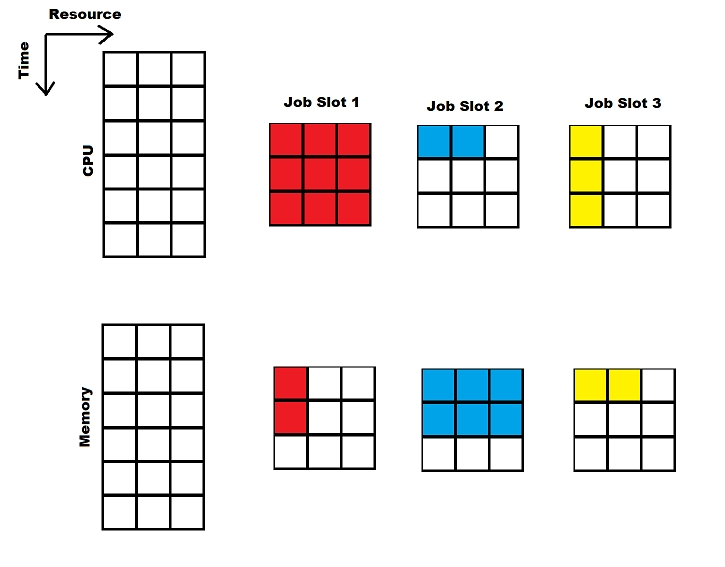
\includegraphics[width=0.5\linewidth]{rm.png}
    \caption{Ví dụ về quản lý tài nguyên với hai loại tài nguyên và ba công việc đang chờ xử lý}
    \label{fig:enter-label}
\end{figure}  

\subsubsection{Thách thức trong quản lý tài nguyên}
\hspace{0.5cm}Quản lý tài nguyên trong các hệ thống máy tính đòi hỏi cân bằng các mục tiêu phức tạp và thường mâu thuẫn, bao gồm tối đa hóa hiệu quả, giảm thiểu độ trễ, và tối ưu hóa việc sử dụng tài nguyên\cite{mao2017resource}. Một số thách thức phổ biến bao gồm:  

\begin{enumerate}[1. ]
    \item \textbf{Sự phức tạp của hệ thống và môi trường động:}
    Các hệ thống hiện đại như cụm máy tính, nền tảng đám mây, và hạ tầng mạng vốn rất phức tạp. Chúng yêu cầu các quyết định được đưa ra trong môi trường thay đổi liên tục, nơi các biến như nhu cầu tài nguyên, nhiễu, và tải hệ thống thay đổi không ngừng.  

    \item \textbf{Ra quyết định trong thời gian thực:}
    Việc phân bổ tài nguyên thường cần được thực hiện trực tuyến, với thời gian tính toán hạn chế và dữ liệu đầu vào có thể không đầy đủ hoặc bị nhiễu. Ví dụ, các nền tảng phát trực tuyến video phải thích ứng với băng thông biến động để đảm bảo phát lại mượt mà.  

    \item \textbf{Ràng buộc đa chiều:}
    Nhu cầu tài nguyên mang tính đa chiều, bao gồm các yếu tố như chu kỳ CPU, không gian bộ nhớ, băng thông I/O, và dung lượng lưu trữ. Phân bổ tài nguyên một cách tối ưu trên các chiều này là một thách thức tổ hợp.  

    \item \textbf{Các chỉ số hiệu suất:}
    Các chỉ số như thời gian hoàn thành công việc, thông lượng hệ thống, và hiệu suất đuôi (tail performance) rất khó để tối ưu hóa đồng thời. Thêm vào đó, mức độ quan trọng của chúng có thể thay đổi tùy theo khối lượng công việc hoặc yêu cầu hệ thống.  
\end{enumerate}  

\subsubsection{Ứng dụng của 2DCSP trong quản lý tài nguyên}  
\hspace{0.5cm}Khung làm việc của 2DCSP giải quyết các thách thức này bằng cách xem việc phân bổ tài nguyên như một bài toán cắt gọt, trong đó mục tiêu là sắp xếp các nhu cầu tài nguyên vào các nguồn lực sẵn có một cách hiệu quả. Quy trình bao gồm các bước sau:  

\begin{enumerate}
    \item \textbf{Mô hình hóa hồ sơ tài nguyên: } 
    Mỗi công việc hoặc tác vụ được biểu diễn dưới dạng một "miếng cắt" hai chiều với các yêu cầu tài nguyên trên nhiều chiều (ví dụ: CPU và bộ nhớ). Các miếng cắt này được sắp xếp vào "nguồn tài nguyên," tương tự như cách phân bổ vật liệu trong bài toán 2DCSP truyền thống.  

    \item \textbf{Mục tiêu tối ưu hóa:} 
    Mục tiêu là giảm thiểu lãng phí tài nguyên trong khi đảm bảo công việc được hoàn thành đúng hạn. Chẳng hạn, trong một kịch bản lập lịch cho cụm máy tính, điều này đồng nghĩa với việc giảm thiểu các khối tài nguyên không sử dụng và đạt được thời gian hoàn thành công việc thấp (job slowdown).  

    \item \textbf{Phương pháp tiếp cận thuật toán: }
    \begin{itemize}
        \item \textbf{Các phương pháp heuristic:} Các thuật toán heuristic truyền thống như chiến lược khớp trước (first-fit) và khớp tốt nhất (best-fit) được điều chỉnh để xử lý các ràng buộc tài nguyên đa chiều.
    \end{itemize}  

    \item \textbf{Mô phỏng và xác nhận:}  
    Các ma trận phân bổ tài nguyên và hồ sơ công việc được sử dụng để mô phỏng kết quả lập lịch. Quy trình này đảm bảo rằng các giải pháp đề xuất đáp ứng các yêu cầu và ràng buộc thực tế.  

    \item \textbf{Triển khai trong các hệ thống thời gian thực:  }
    Các giải pháp 2DCSP nâng cao có thể được triển khai trong các hệ thống quản lý tài nguyên thời gian thực. Ví dụ, trong điện toán đám mây, chúng có thể phân bổ máy ảo vào các máy chủ vật lý, cân bằng khối lượng công việc và giảm thiểu sự phân mảnh.  
\end{enumerate}  

\subsubsection{Lợi ích thực tiễn}  
\hspace{0.5cm}Việc tích hợp 2DCSP vào quản lý tài nguyên mang lại nhiều lợi ích:  

\begin{itemize}
    \item \textbf{Tăng cường sử dụng tài nguyên:} Bằng cách giảm thiểu phân mảnh và lãng phí, hệ thống có thể xử lý nhiều công việc hơn trong cùng một lượng tài nguyên.  
    \item \textbf{Cải thiện hiệu suất hệ thống:} Phân bổ tài nguyên tối ưu giúp giảm thời gian hoàn thành công việc và tuân thủ tốt hơn các thỏa thuận cấp dịch vụ (SLA).  
    \item \textbf{Tính linh hoạt và khả năng mở rộng:} Bản chất thích ứng của các phương pháp 2DCSP cho phép hệ thống xử lý khối lượng công việc đa dạng và phản ứng với các thay đổi động trong nhu cầu.  
    \item \textbf{Giảm chi phí vận hành:} Sử dụng tài nguyên hiệu quả giúp giảm tiêu thụ năng lượng và chi phí phần cứng, mang lại khoản tiết kiệm đáng kể.  
\end{itemize}  


\subsection{Bảng mạch in}

\hspace{0.5cm}Bài toán cắt tấm 2 chiều (2D Cutting Stock Problem - 2DCSP) là một phần cốt lõi trong chiến lược tối ưu hóa của nhiều ngành công nghiệp đòi hỏi sự chính xác và hiệu quả trong việc sử dụng nguyên liệu. Một trong những ứng dụng nổi bật nhất của 2DCSP nằm trong lĩnh vực cắt bảng mạch, một quá trình quan trọng trong sản xuất thiết bị điện tử \cite{ulutas2023effectiveness}. Tính phức tạp và tầm quan trọng của sản xuất bảng mạch đã làm cho 2DCSP trở thành một công cụ không thể thiếu nhằm giải quyết các vấn đề về lãng phí nguyên liệu, hiệu quả vận hành, và tính bền vững với môi trường.

\subsubsection{Tầm quan trọng của tối ưu hóa trong cắt bảng mạch}
\hspace{0.5cm}Bảng mạch đóng vai trò là nền tảng của các thiết bị điện tử hiện đại, đòi hỏi sự chú ý tỉ mỉ trong sản xuất. Quá trình cắt, nhằm định hình các tấm bảng mạch in (PCB) lớn thành các đơn vị nhỏ hơn, đối mặt với nhiều thách thức độc đáo \cite{ulutas2023effectiveness}. Các thách thức này bao gồm:

\begin{enumerate}[1.  ]
    \item Tối đa hóa sử dụng nguyên liệu: Chi phí cao của vật liệu PCB đòi hỏi các chiến lược giảm thiểu lãng phí, đặc biệt trong bối cảnh các thực hành sản xuất bền vững ngày càng được chú trọng.
    \item Đảm bảo độ chính xác về hình học: Mỗi đường cắt phải hoàn toàn phù hợp với các thông số thiết kế của bảng để duy trì tính toàn vẹn của mạch và kết nối.
    \item Xử lý các hình dạng đa dạng và bất thường: Không giống như các hình dạng đơn giản như hình chữ nhật hoặc hình vuông, bảng mạch thường yêu cầu các hình dạng không chuẩn, làm tăng đáng kể độ phức tạp của quá trình tối ưu hóa.
    \item Cân bằng giữa tốc độ và độ chính xác: Với nhu cầu ngày càng tăng về các sản phẩm điện tử, các nhà sản xuất phải tăng quy mô sản xuất trong khi vẫn đảm bảo chất lượng cao.
\end{enumerate}

\subsubsection{Cách 2DCSP giải quyết các thách thức trong cắt bảng mạch}
Phương pháp 2DCSP cung cấp một khung giải pháp mạnh mẽ để xử lý các thách thức này thông qua sự kết hợp giữa mô hình hóa toán học, thiết kế thuật toán, và hiệu quả tính toán. Việc tích hợp 2DCSP vào cắt bảng mạch bao gồm các bước sau:

\begin{figure}[!htp]
    \centering
    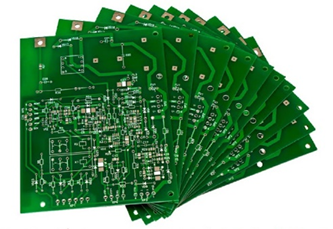
\includegraphics[width=0.3\linewidth]{circuits.png}
    \caption{Mạch điện tử}
    \label{fig:enter-label}
\end{figure}

\begin{enumerate}[1.]
    \item Chuẩn bị dữ liệu và định nghĩa bài toán:
    \begin{itemize}
        \item Các thông số đầu vào như kích thước của vật liệu PCB thô, các hình dạng và kích thước yêu cầu, khả năng của dụng cụ cắt, và các ràng buộc về bố cục được thu thập cẩn thận.
        \item Các thông số này được chuyển đổi thành một biểu diễn chính thức của bài toán 2DCSP, trong đó mục tiêu là giảm thiểu lãng phí trong khi đáp ứng các yêu cầu sản xuất.
    \end{itemize}
    

    \item Các giải pháp thuật toán:
    \begin{itemize}
        \item Một loạt các phương pháp tối ưu hóa có thể được áp dụng, từ các thuật toán chính xác như lập trình tuyến tính và kỹ thuật branch-and-bound đến các phương pháp heuristic và metaheuristic, bao gồm thuật toán di truyền, làm nguội mô phỏng, và tối ưu hóa đàn hạt.
        \item Các thuật toán này đánh giá vô số mẫu cắt tiềm năng, xác định các cấu hình đạt hiệu suất sử dụng nguyên liệu gần tối ưu hoặc tối ưu.
    \end{itemize}


    \item Mô phỏng và cải tiến lặp:
     \begin{itemize}
        \item Khi các giải pháp ban đầu được tạo ra, các mô phỏng sẽ kiểm tra tính khả thi của chúng, xét đến các ràng buộc thực tế như dung sai của máy móc và các khuyết tật vật liệu có thể xảy ra.
        \item Phản hồi từ các mô phỏng được sử dụng để tinh chỉnh các mẫu, đảm bảo đầu ra cuối cùng vừa hiệu quả vừa có thể thực hiện.
    \end{itemize}

    \item Triển khai trong sản xuất:
     \begin{itemize}
        \item Các mẫu đã được xác nhận được tích hợp vào phần mềm của máy cắt, dẫn dắt quá trình cắt vật lý với sự can thiệp tối thiểu của con người.
        \item Các hệ thống tiên tiến tích hợp điều chỉnh thời gian thực, thích ứng động các mẫu trong trường hợp xảy ra các vấn đề bất ngờ, chẳng hạn như sự không đồng nhất của vật liệu.
    \end{itemize}
\end{enumerate}

\subsubsection{Lợi ích đo lường được từ việc áp dụng 2DCSP trong cắt bảng mạch}
\hspace{0.5cm}Việc áp dụng thực tế của 2DCSP đã mang lại những cải thiện mang tính cách mạng trong sản xuất bảng mạch. Các lợi ích đáng chú ý bao gồm:

\begin{figure}[!htp]
    \centering
    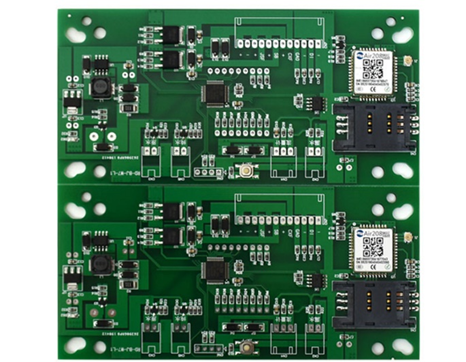
\includegraphics[width=0.5\linewidth]{circuit.png}
    \caption{Thành phần của bảng mạch điện tử}
    \label{fig:enter-label}
\end{figure}

\begin{itemize}
    \item Giảm lãng phí đáng kể: Các nhà sản xuất báo cáo giảm tới 25\% lượng lãng phí nguyên liệu khi sử dụng các mẫu cắt tối ưu so với phương pháp truyền thống.
    \item Tiết kiệm chi phí: Lượng lãng phí giảm dẫn đến chi phí nguyên liệu thấp hơn, trong khi các mẫu cắt hiệu quả cũng giảm thiểu hao mòn máy móc và tiêu thụ năng lượng.
    \item Tăng cường tính linh hoạt: Tính thích ứng của các mô hình 2DCSP cho phép các nhà sản xuất xử lý nhiều loại đơn đặt hàng, từ các thiết kế tiêu chuẩn đến các bố cục được tùy chỉnh cao, mà không làm giảm hiệu quả.
    \item Cải thiện tác động môi trường: Bằng cách giảm thiểu lãng phí và tối ưu hóa việc sử dụng tài nguyên, 2DCSP góp phần vào các thực hành sản xuất bền vững, phù hợp với các nỗ lực toàn cầu nhằm giảm dấu chân carbon của ngành công nghiệp.
\end{itemize}
